\documentclass[conference]{IEEEtran}

\usepackage{cite}
\usepackage{url}
\usepackage[cmex10]{amsmath}
\usepackage[ruled]{algorithm2e}
\usepackage{algorithmic}
\usepackage{amssymb}
\usepackage{multirow}
\interdisplaylinepenalty=2500

% *** GRAPHICS RELATED PACKAGES ***
%

% % % % % MACROS  % % % % % % %
\newcommand{\imagepath}{../../images/diagrams/}
\newcommand{\colwidth}{2.6in}
% % % % % % % % % % % % % % % %

%\ifCLASSINFOpdf
  \usepackage[pdftex]{graphicx}
  % declare the path(s) where your graphic files are
  % ../.. is the GeocronDocuments directory
  \graphicspath{{../../images/external/location_routing}{../../images/}}
  % and their extensions so you won't have to specify these with
  % every instance of \includegraphics
  \DeclareGraphicsExtensions{.pdf,.png}
%\else
  % or other class option (dvipsone, dvipdf, if not using dvips). graphicx
  % will default to the driver specified in the system graphics.cfg if no
  % driver is specified.
  % \usepackage[dvips]{graphicx}
  % declare the path(s) where your graphic files are
  % \graphicspath{{../eps/}}
  % and their extensions so you won't have to specify these with
  % every instance of \includegraphics
  % \DeclareGraphicsExtensions{.eps}
%\fi
\usepackage[caption=false,font=footnotesize]{subfig}
\hyphenation{}
\begin{document}
%
% can use linebreaks \\ within to get better formatting as desired
\title{CS237 Project final report}

\author{\IEEEauthorblockN{Kyle E. Benson and Zhipeng Huang}
\IEEEauthorblockA{Donald Bren School of Information and Computer Sciences\\
University of California, Irvine\\
Irvine, California 92697\\
Email: kebenson@uci.edu, zhipengh@uci.edu}}

% use for special paper notices
\IEEEspecialpapernotice{(Project Report for CS 237 - Distributed Systems Middleware)}


\maketitle


\section{Algorithm}
There are six routing heuristic algorithms that have been tested and compared in the simulation: orthogonal distant path heuristic, new region heuristic, new angle path heuristic, distant-dependent path heuristic, furthest first path heuristic and closest first path heuristic.
The New Angle, Distance-Dependent, and Furthest-First heuristics are new contributions from this project.

% % %
%
\subsection{Orthogonal Distant Path Heuristic}
The intuition of this heuristic is to avoid the straight path, without diverging from it too much.  It strikes a middle ground by choosing a path at an ideal angle of $45^{\circ}$, which makes the angle at the top orthogonal, hence the name.
\begin{algorithm}
\DontPrintSemicolon
\SetKwBlock{Begin}{begin}{end}
\SetAlgoLined
\SetAlgoLongEnd
\scriptsize
\Begin{
\tcc*[l]{Sensor, overlay and server node are a, c, b respectively}
$idealDist = |0.5 \cdot dist(a,b)|$\;
$perpDist = |\sin (angA) \cdot dist(a,c)|$\;
\lIf{$angA > \frac{\pi}{2}$ {\bf or} $angA + angC < \frac{\pi}{2}$ {\bf or} $perpDist > dist(a,b)$} {$likelihood = 0$\;}
\lElse {$likelihood = 0.5 \cdot (( 1.0 - (||perpDist|-|idealDist|| / idealDist)^{2}) + ( 1.0 - (|\frac{\pi}{2} - angC| / \frac{\pi}{2})^{2}))$\;}
}
\caption{}
\small
\end{algorithm}

\begin{figure}
\centering
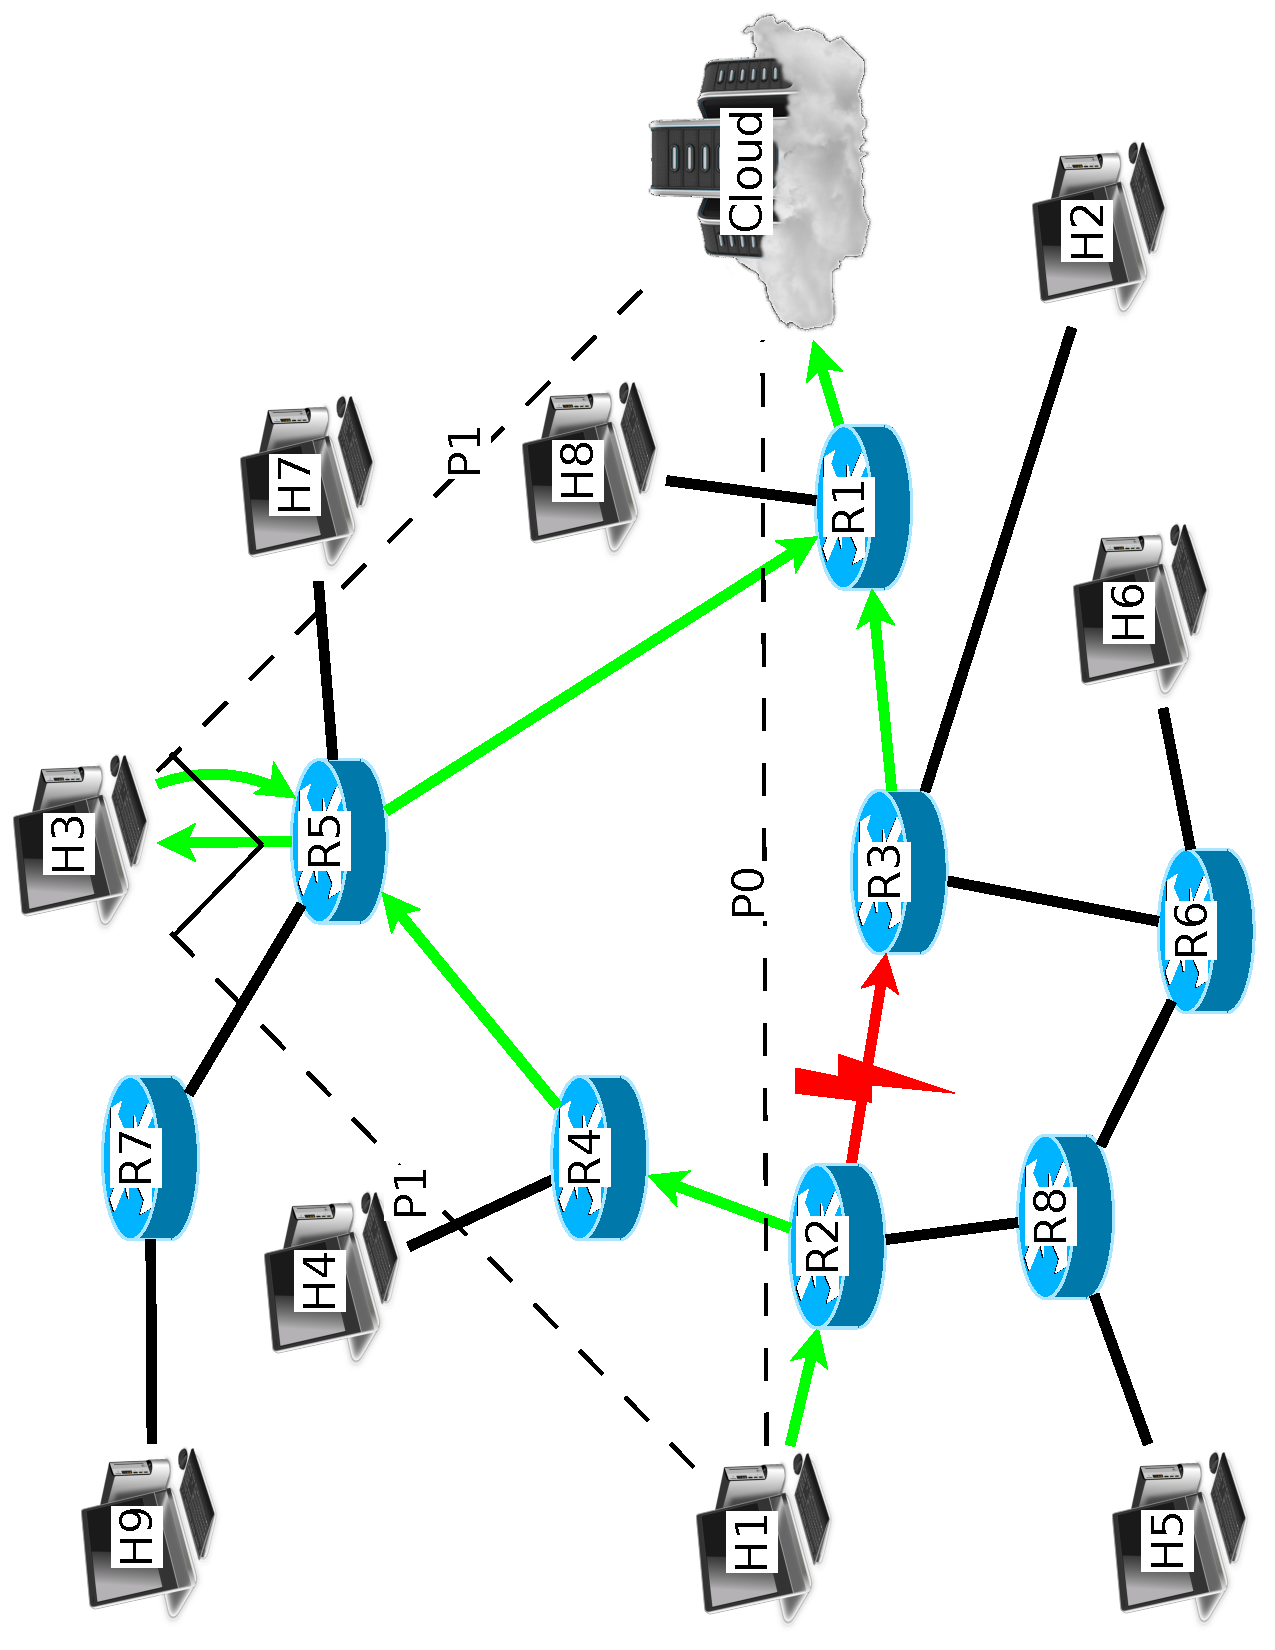
\includegraphics[scale=0.25,angle=-90]{../../images/diagrams/angular_path}
\caption{Orthogonal Distant Path Heuristic}
\end{figure}

% % % % % % % % %
%
\subsection{New Region Heuristic}
The intuition of this heuristic is to avoid regions that have been previously attempted unsuccessfully.  We assume that no further attempts to contact such a region will succeed.
\begin{algorithm}
\DontPrintSemicolon
\SetKwBlock{Begin}{begin}{end}
\SetAlgoLined
\SetAlgoLongEnd
\scriptsize
\Begin{
%\tcc*[l]{Discover any node that has not been discoverd in this region}
\lIf{$peer.region \in regionsAttempted$} {$likelihood = 0$\;}
\lElse {$likelihood = 1.0$\;}
}
\caption{}
\small
\end{algorithm}

\begin{figure}
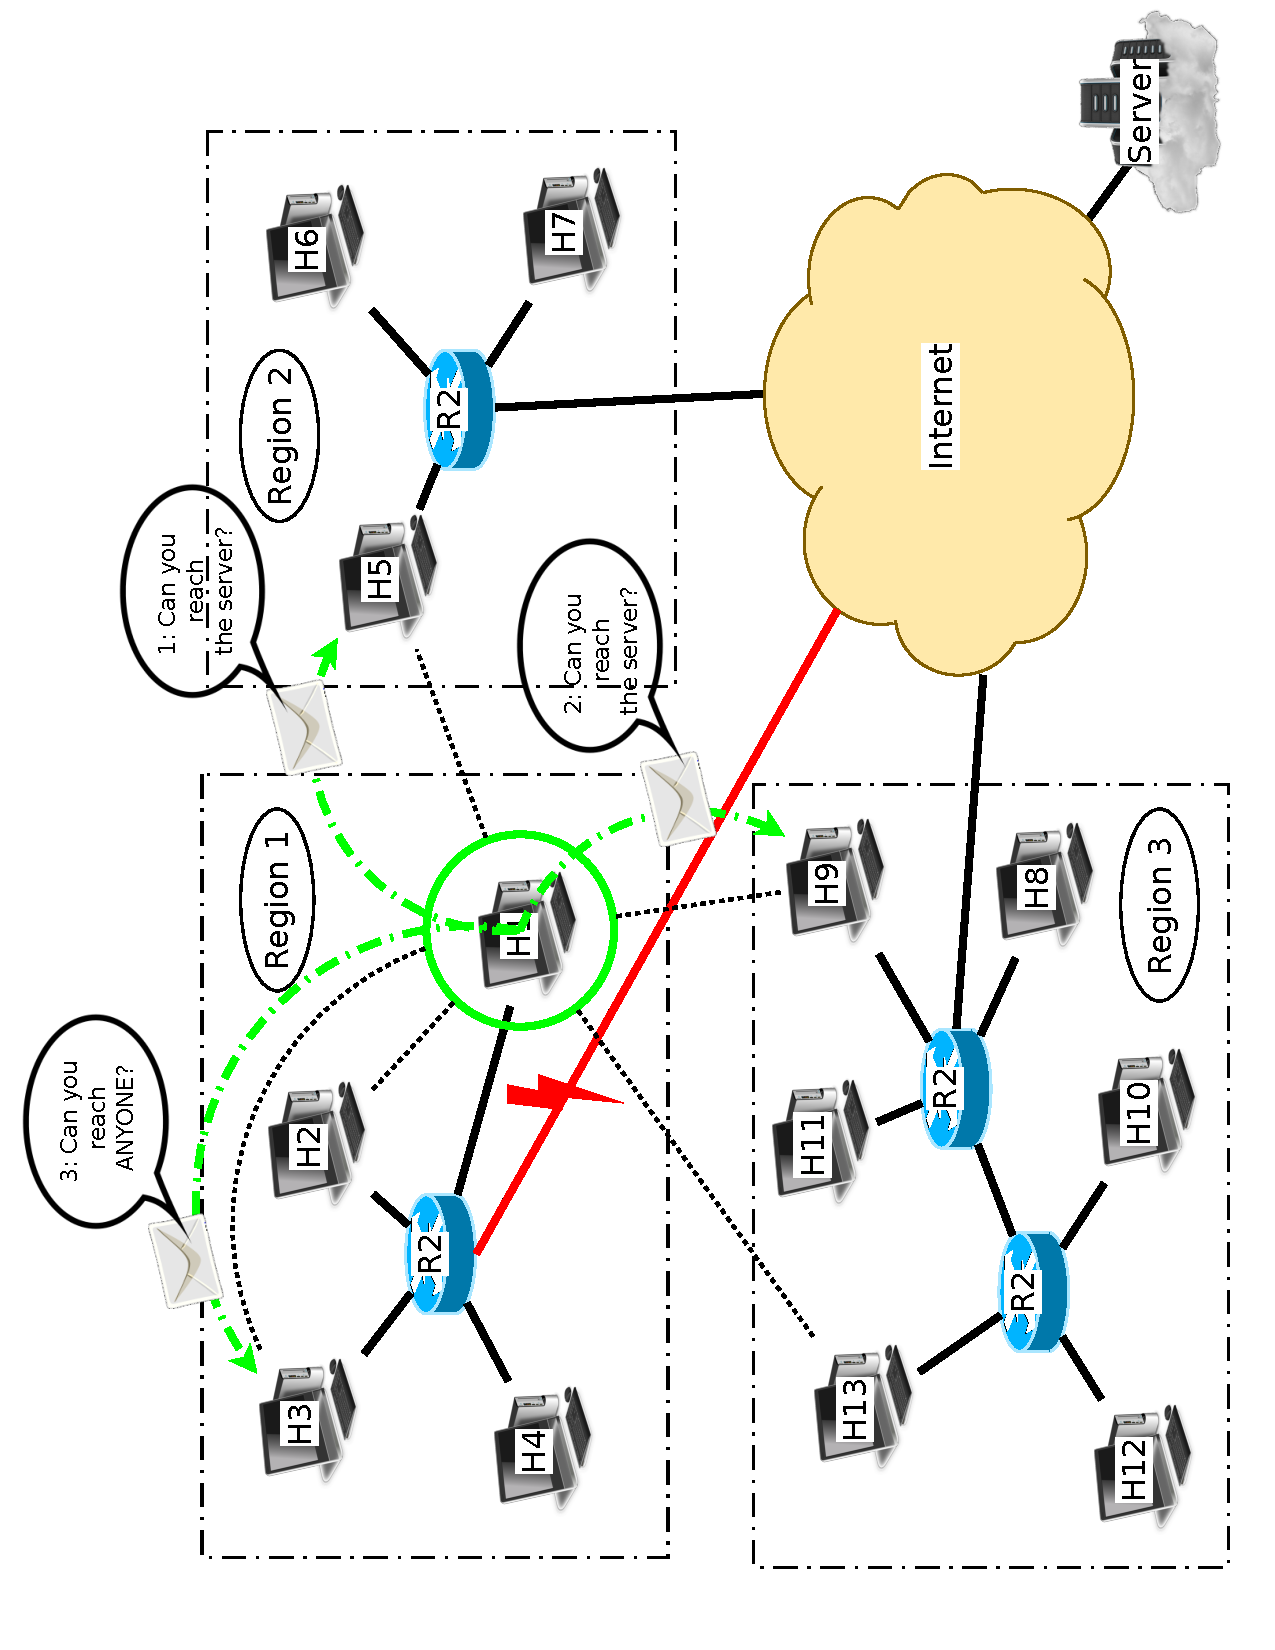
\includegraphics[scale=0.25,angle=-90]{../../images/diagrams/new_region_all}
\caption{New Region Heuristic}
\end{figure}

% % %
%
\subsection{New Angle Path Heuristic}
This heuristic attempts paths along new angles different from the ones previously attempted.
\begin{algorithm}
\DontPrintSemicolon
\SetKwBlock{Begin}{begin}{end}
\SetAlgoLined
\SetAlgoLongEnd
\scriptsize
\Begin{
%\tcc*[l]{The angle could be either acute or obtuse.}
$angle = Angle(overlay,server)$\;
\lIf{$angle = \pi$ {\bf or} $angle = 0$} {$initLikelihood = 0$\;}
\lElseIf{$angle < \pi$} {$initLikelihood = \cos (angle - \frac{\pi}{4})$\;}
\lElseIf{$angle > \pi$} {$initLikelihood = \cos (2 \cdot ((2\pi - angle) - \frac{\pi}{4})/3)$\;}
\lForEach {$path \in pathsAttempted$} {$thisLikelihood = |\frac{\sin (angle)}{2}|$\;} {$newLikelihood *= thisLikelihood$\;}
%\tcc*[l]{aggregate likelihoods to make punishments on wrong choices}
}
\caption{}
\small
\end{algorithm}

\begin{figure}
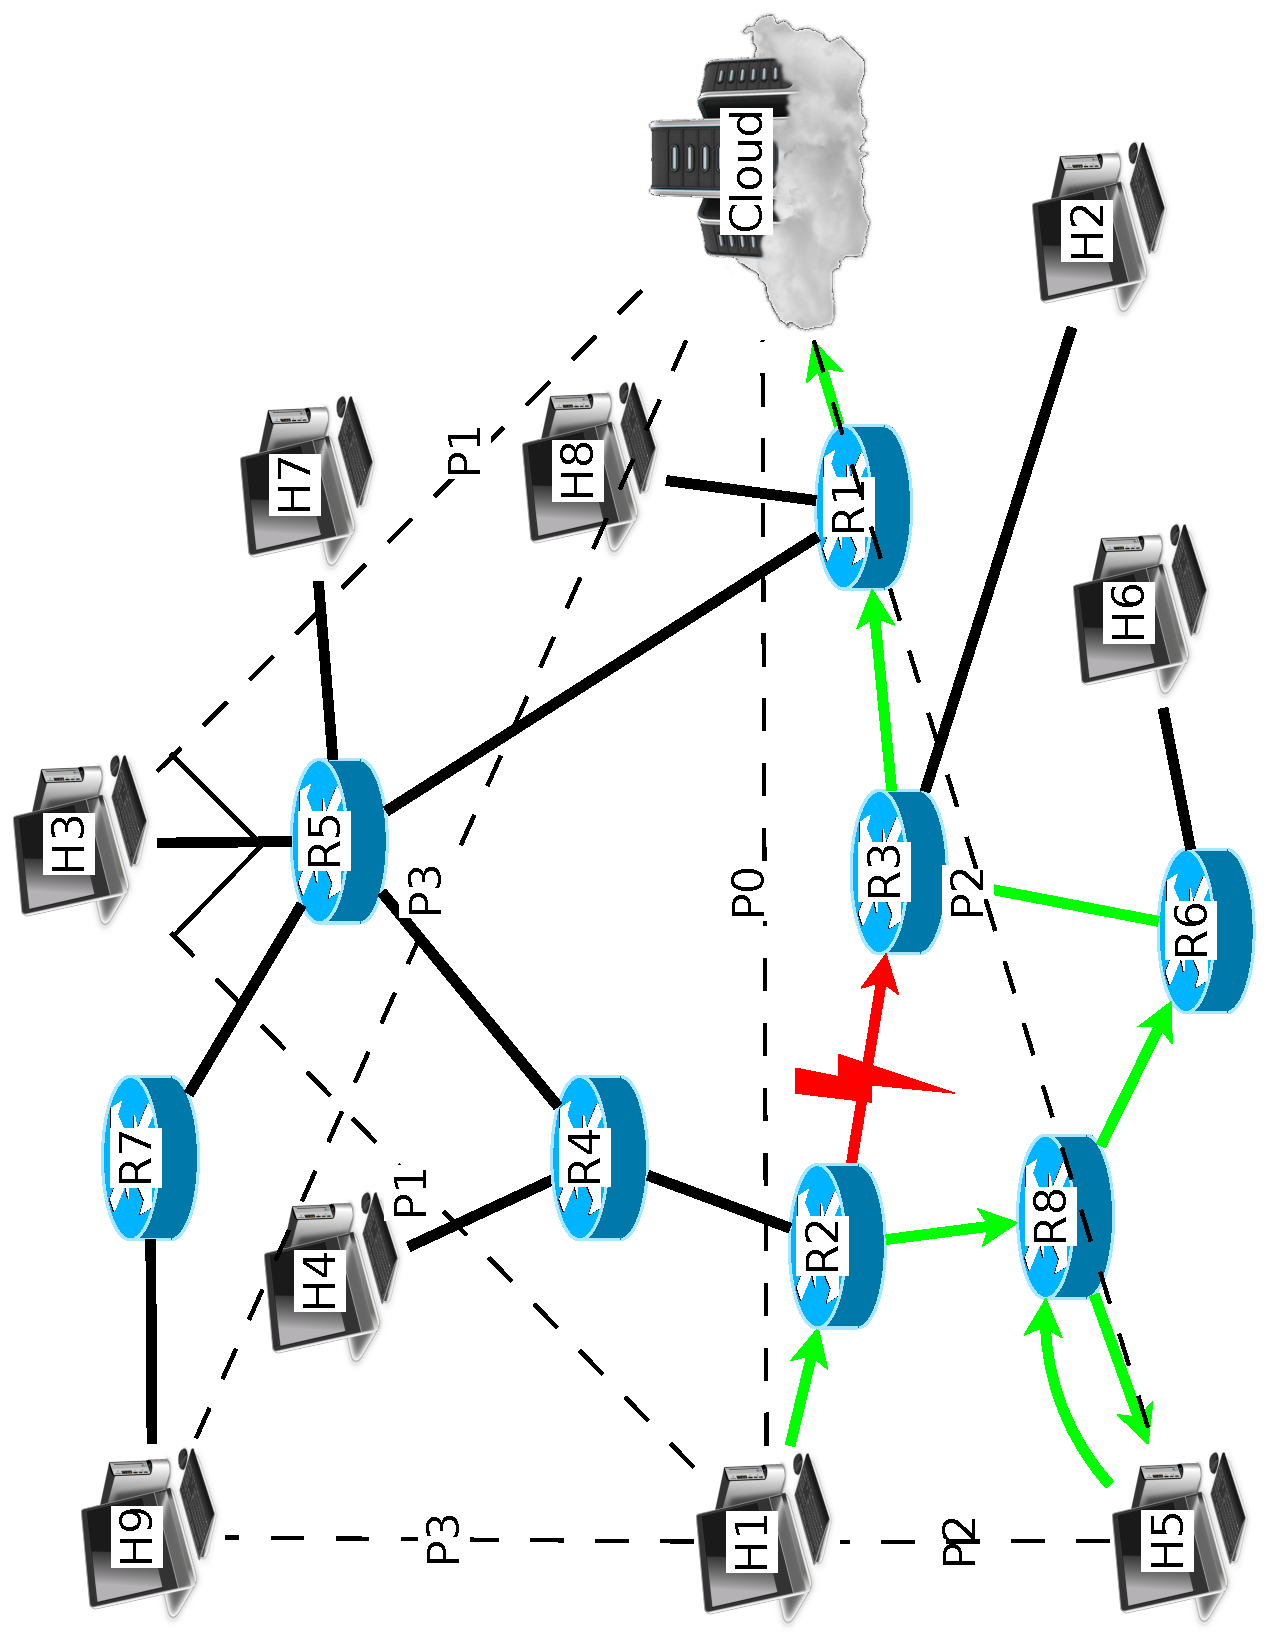
\includegraphics[scale=0.25,angle=-90]{../../images/diagrams/new_angle}
\caption{New Angle Path Heuristic}
\end{figure}

% % % %
%
\subsection{Distance-Dependent Path Heuristic}
This heuristic attempts paths that use overlay nodes at an ideal distance from the sensor.  This ideal distance is chosen as a radius that reaches half-way to the server.
\begin{algorithm}
\DontPrintSemicolon
\SetKwBlock{Begin}{begin}{end}
\SetAlgoLined
\SetAlgoLongEnd
\scriptsize
%\SetAlgoSkip{bigskip}
%\SetAlgoInsideSkip{medskip}
%$/*Initialization*/$\;
\Begin{
\tcc*[l]{minDist = some reasonably small number}
$idealDist = 0.5 \cdot dist(sensor,server)$
$dist = dist(sensor,overlay)$
\lIf{$dist <= minDist$} {$likelihood = 0$\;}
\lElseIf{$minDist < dist < idealDist$} {$likelihood = dist^{2} / idealDist^{2}$\;}
\lElseIf{$dist >= idealDist$} {$likelihood = idealDist / dist $\;}
}
\caption{}
\small
\end{algorithm}

\begin{figure}
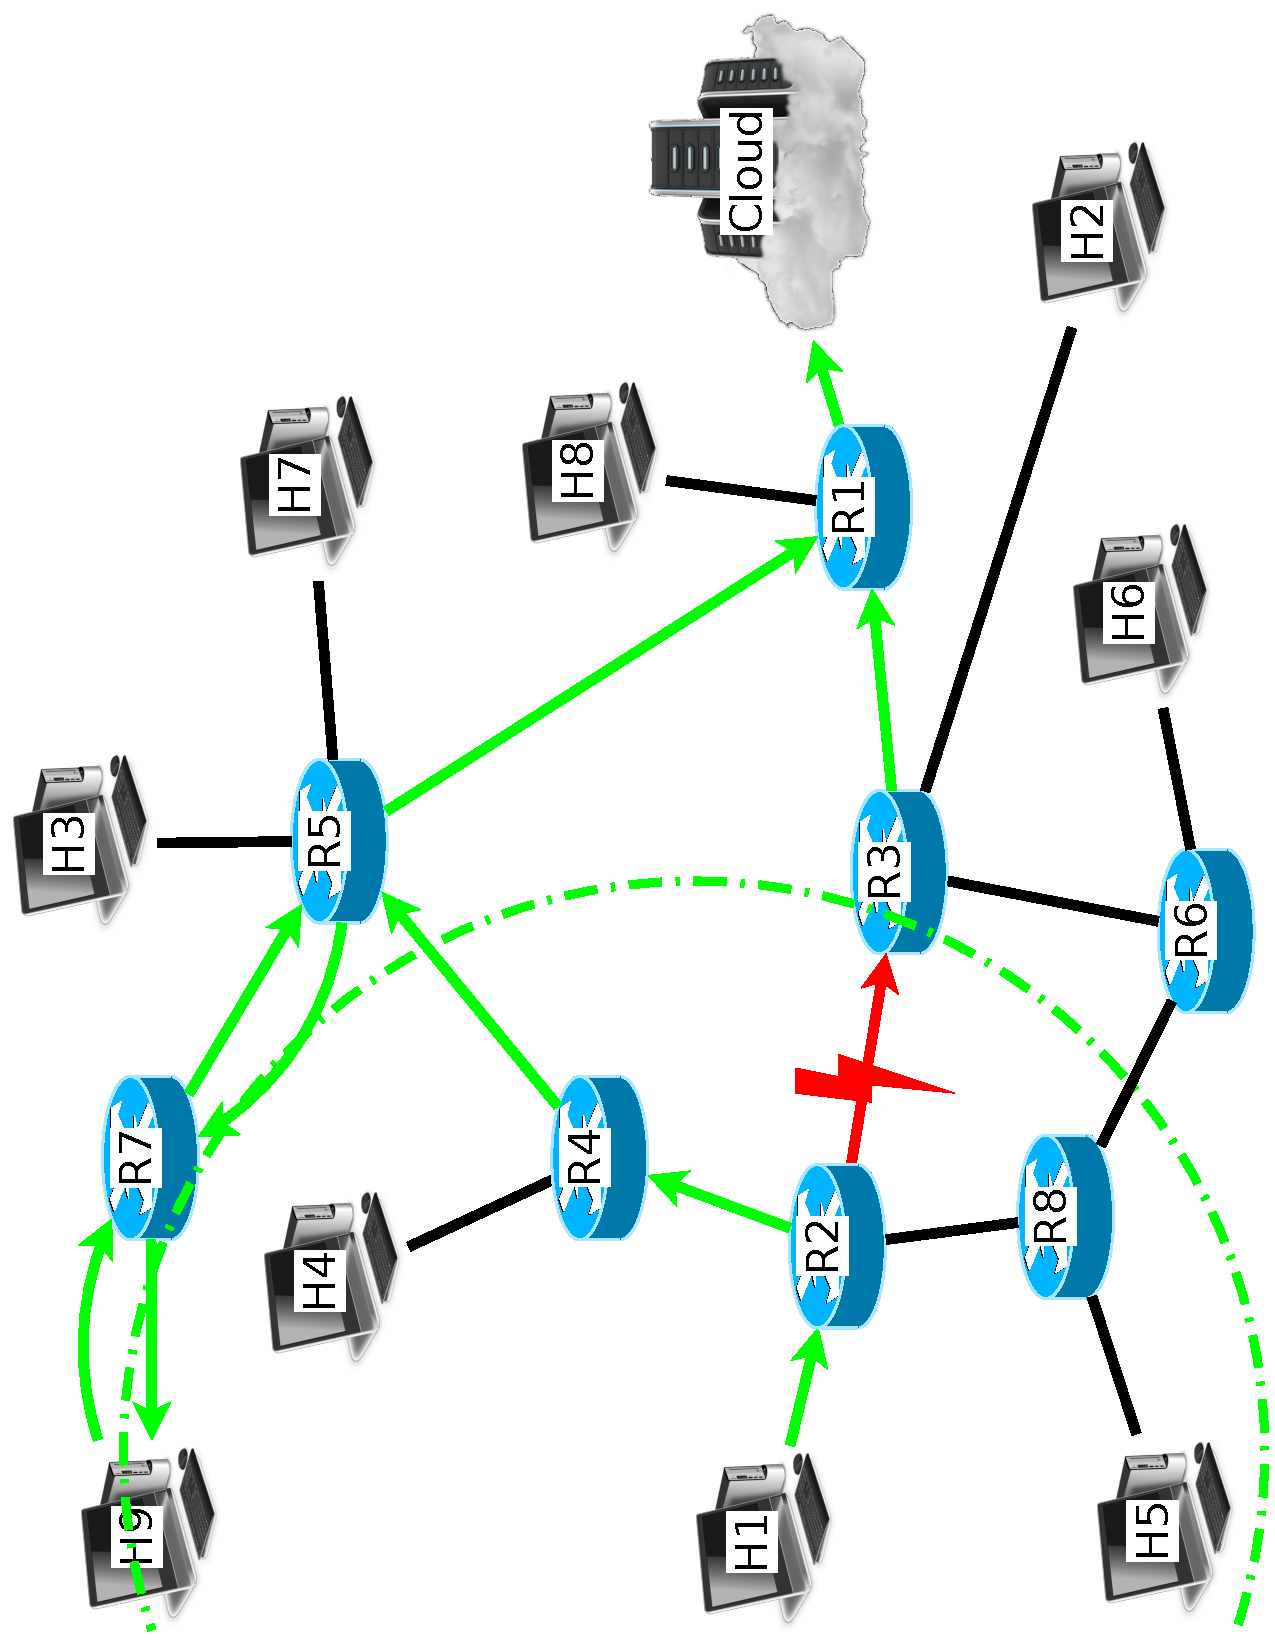
\includegraphics[scale=0.25,angle=-90]{../../images/diagrams/ideal_distant_path}
\caption{Distance-Dependent Path Heuristic}
\end{figure}
% % %
%
\subsection{Furthest First Path Heuristic}
This heuristic considers overlay peers located further away to be more likely candidates.

\begin{algorithm}
\DontPrintSemicolon
\SetKwBlock{Begin}{begin}{end}
\SetAlgoLined
\SetAlgoLongEnd
\scriptsize
\Begin{
\tcc*[l]{minDistance = some constant small number}
\lIf{$dist(a,b) < minDistance$} {$likelihood = 0$\;}
\lElse {$likelihood = (dist(a,b) - minDistance) / dist(a,b) $\;}
}
\caption{}
\small
\end{algorithm}

\begin{figure*}[htbp]
\begin{center}
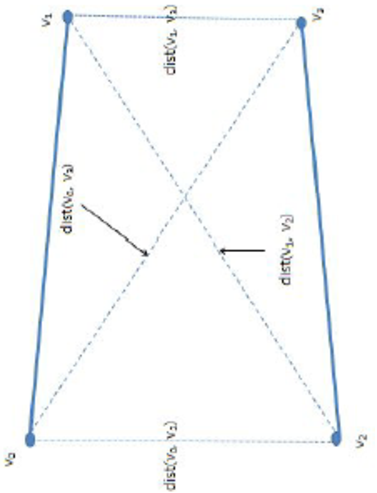
\includegraphics[scale=0.7,angle=-90]{../../images/external/location_routing/path_similarity_two_destinations}
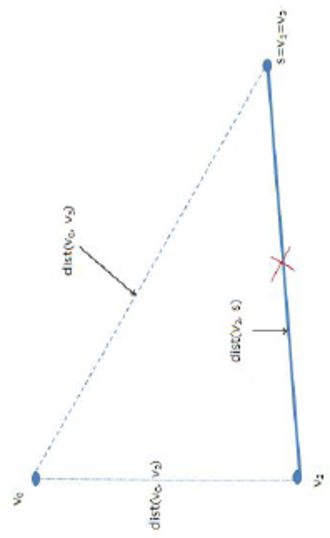
\includegraphics[scale=0.7,angle=-90]{../../images/external/location_routing/path_similarity_one_destination}
\caption{Furthest First Path Heuristic}
\end{center}
\end{figure*}
% % %
%
\subsection{Closest First Path Heuristic}
The intuition of this heuristic is to contact nearby overlay nodes that have found a path out of the local region.  We found, however, that this approach does not always work well in practice, likely due to the path similarity inherent with nearby nodes.
\begin{algorithm}
\DontPrintSemicolon
\SetKwBlock{Begin}{begin}{end}
\SetAlgoLined
\SetAlgoLongEnd
\scriptsize
\Begin{
\tcc*[l]{maxDistance = some constant large number}
\lIf{$dist(a,b) > maxDistance$} {$likelihood = 0$\;}
\lElse {$likelihood = (maxDistance - dist(a,b)) / maxDistance $\;}
}
\caption{}
\small
\end{algorithm}

\begin{figure}
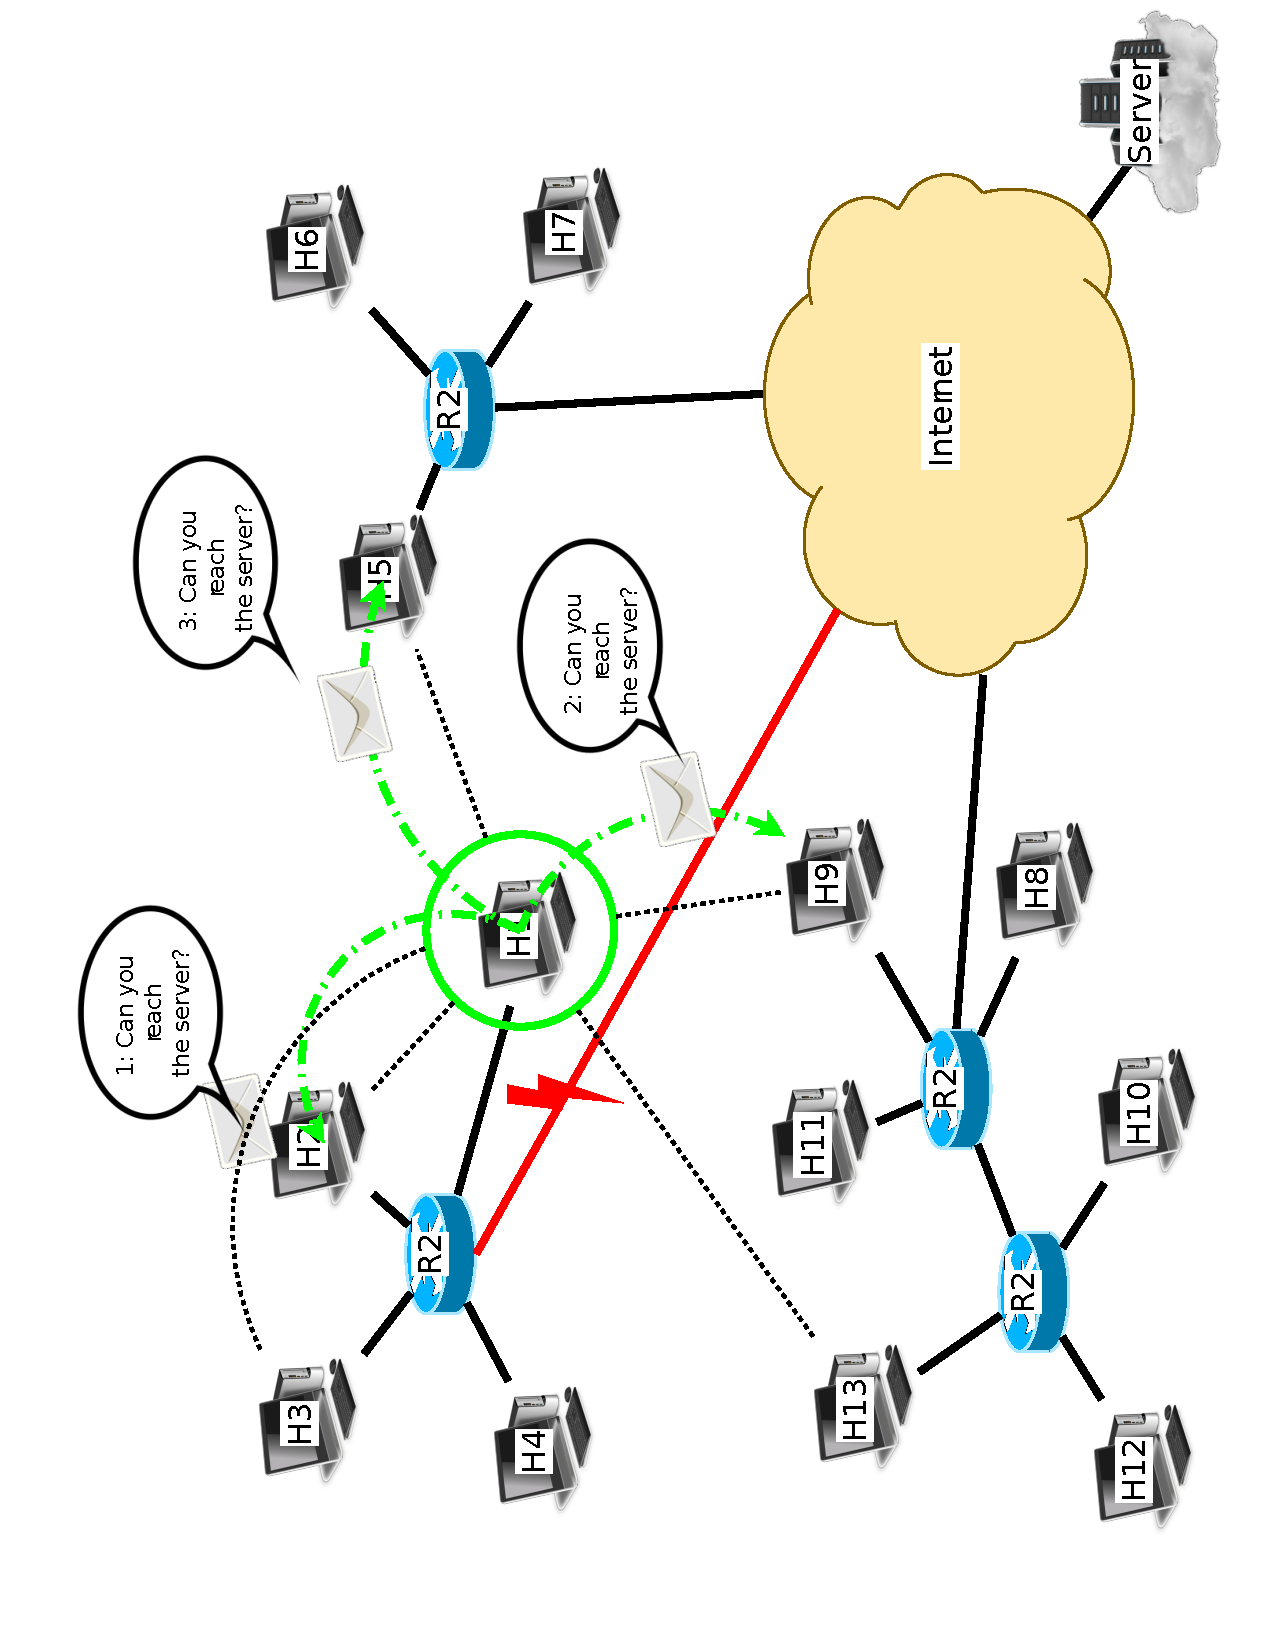
\includegraphics[scale=0.25,angle=-90]{../../images/diagrams/nearest_neighbor}
\caption{Closest First Path Heuristic}
\end{figure}

% % %
%
\section{Conclusion}
In this paper, we described our recent additions to the GeoCRON simulator.
In particular, we:

\begin{itemize}
 \item Switched from Rocketfuel to BRITE for creating ns-3 network topologies
\item Added the New Angle heuristic, which repeatedly tries overlay nodes at diverse angles
\item Added the Furthest-First heuristic, which attempts to contact overlay nodes furthest from the source
\item Added the Distance-Dependent heuristic, which tries to pick overlay nodes at an ideal distance from the source, preferring nodes further away over those close by
\item Defined a new method for assigning regions to nodes in which the region of study is broken up into a grid, where each cell is a constant size
\end{itemize}

We ran simulations on topologies of 10,000 nodes and 25 regions, comparing the peformance of each heuristic with each other.
The results were inconclusive, demonstrating that further refinement and/or combinations of heuristics are necessary to improve the delivery ratio.
For example, the New Angle and Distance-Dependent heuristics may be combined with varying weights to pick nodes both far away from the source as well as along diverse paths.

There are certain other aspects that need to be improved in the future.
First of all, a detailed comparison between the six heuristics should be explored regarding aspects such as difference in convegence time, latency, expected delivery ratio, etc.
Moreover, the purpose of the simulation of the six algorithms should be more clear.

% % %
% %
\section{Results}
\begin{figure}
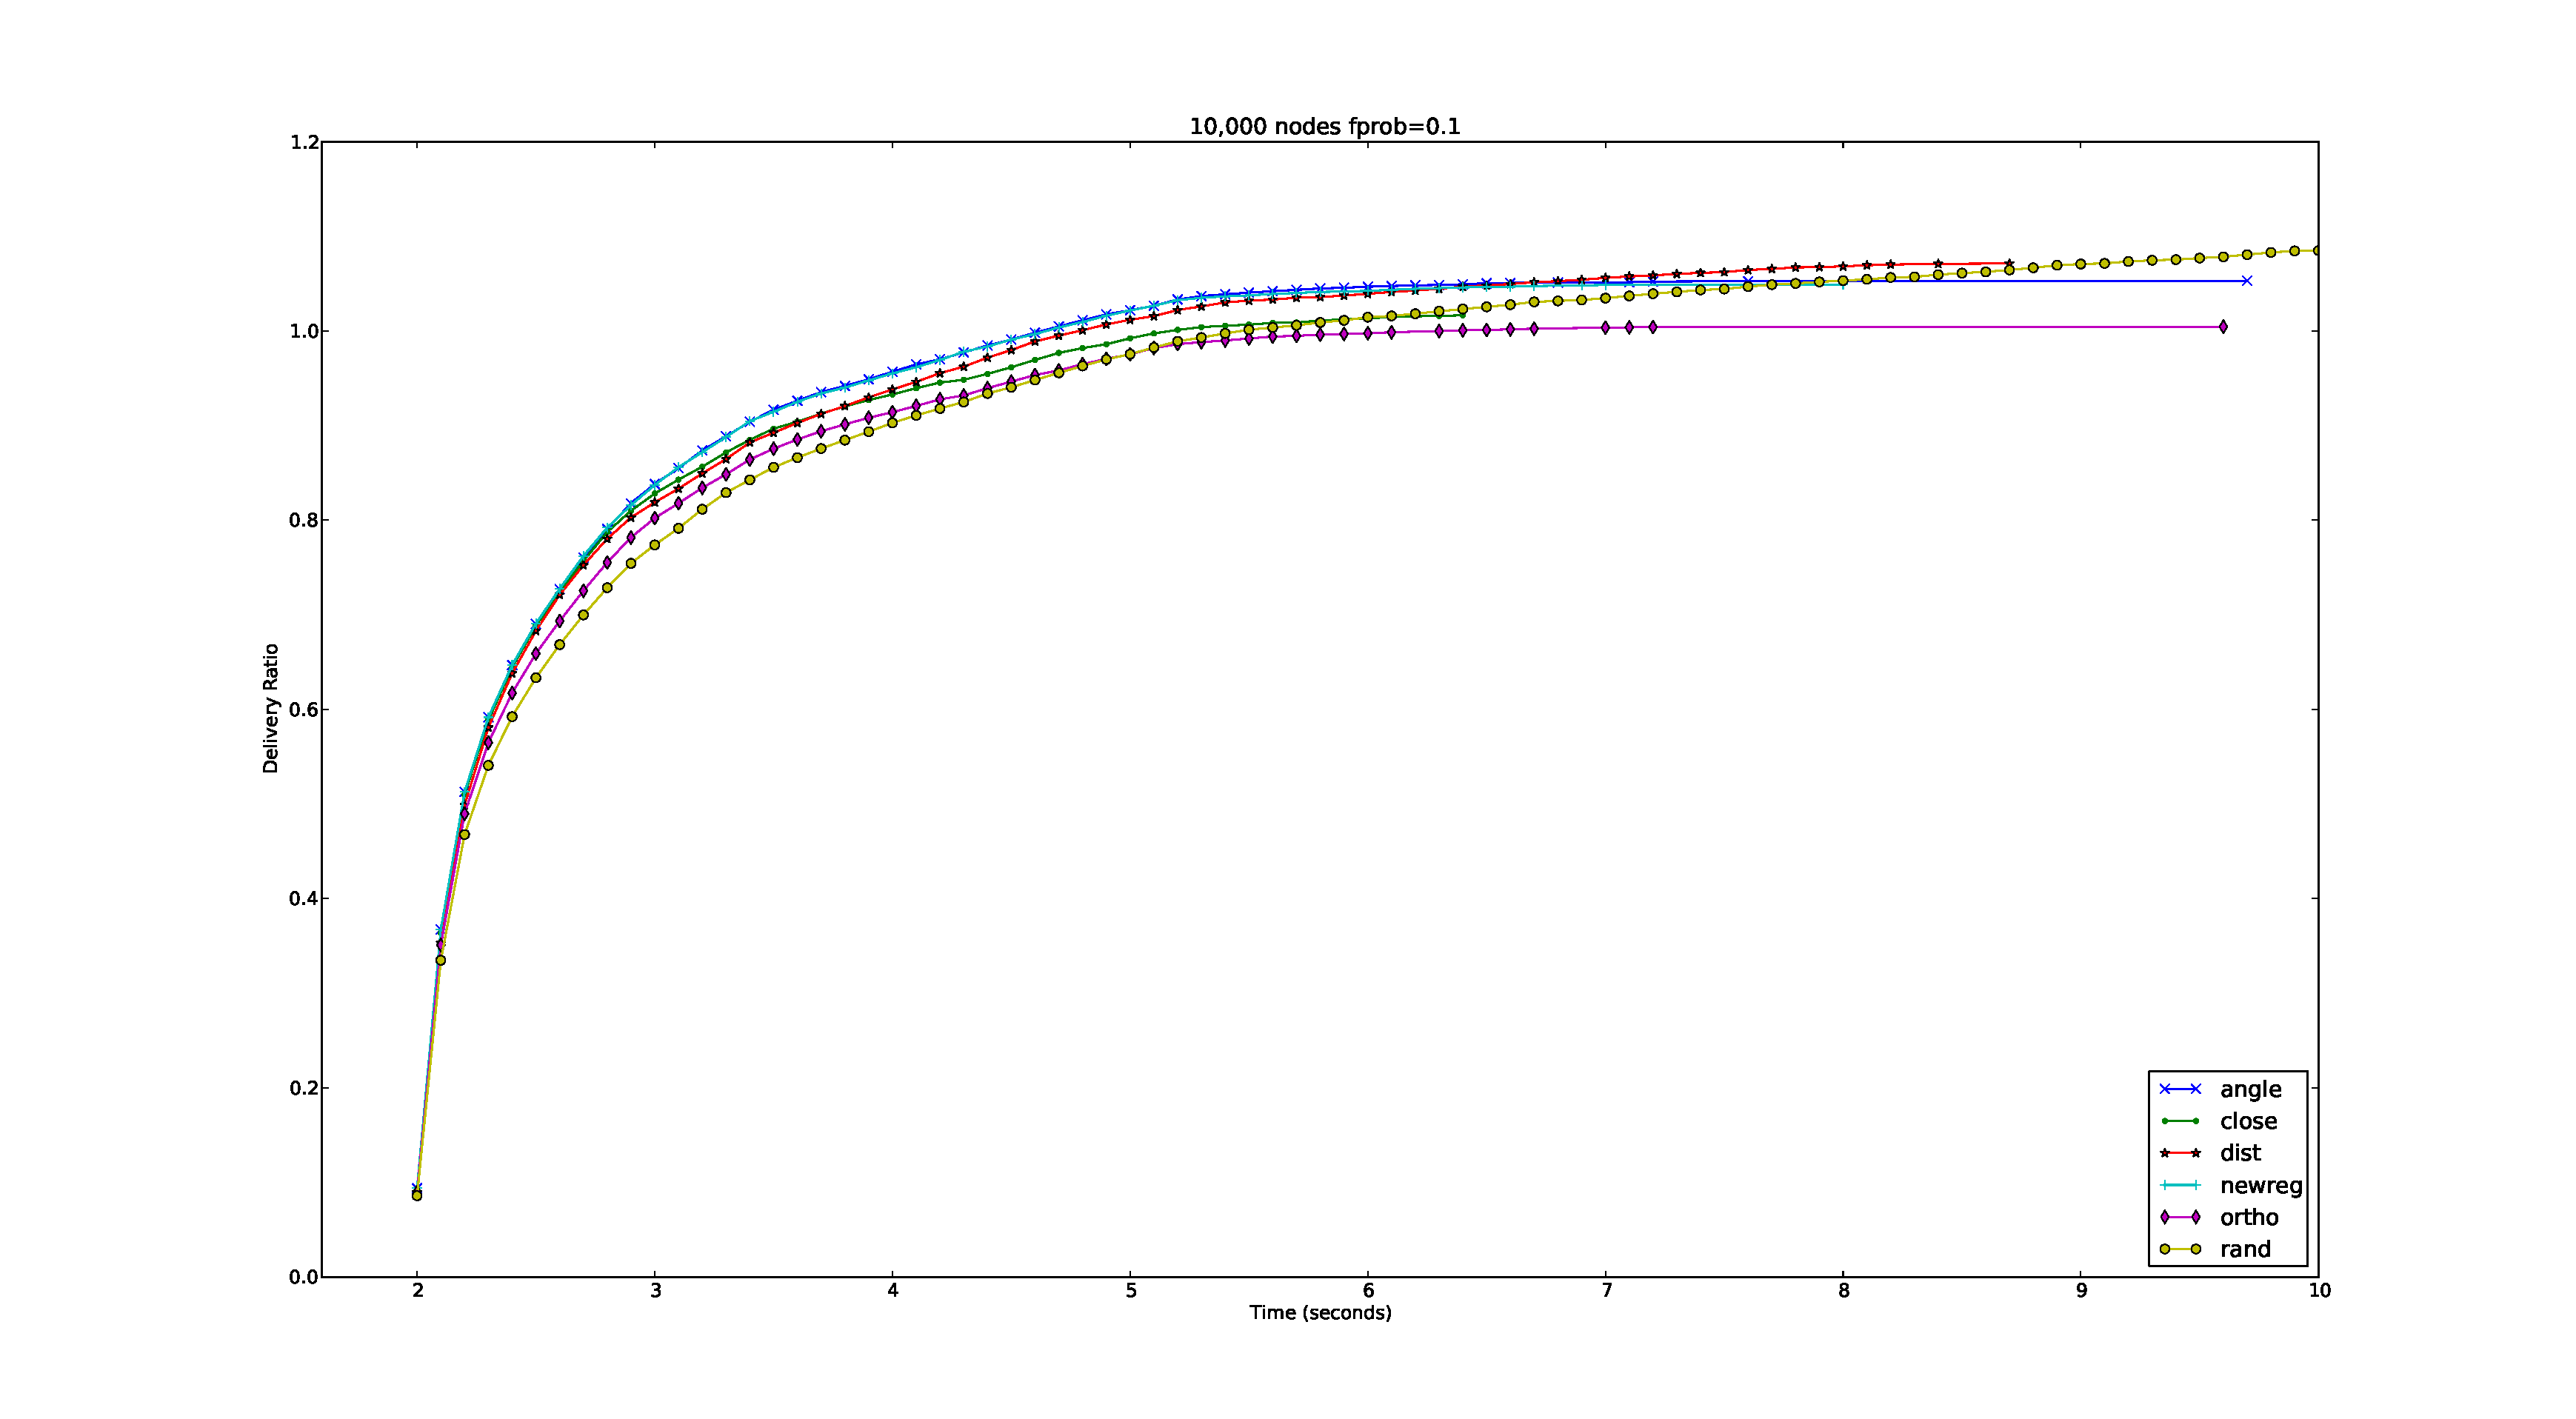
\includegraphics[width=.8\textwidth]{../../images/plots/fprob1}
\vspace{-20pt}
\caption{Delivery ratio of the various heuristics for a failure probability of 0.1.
One can notice the way the heuristics sometimes overcome another's delivery ratio as time evolves and different paths are considered.
NOTE: due to some necessarily aggressive data cleaning, the delivery ratio is exaggerated and skewed.}
\end{figure}
\begin{figure}
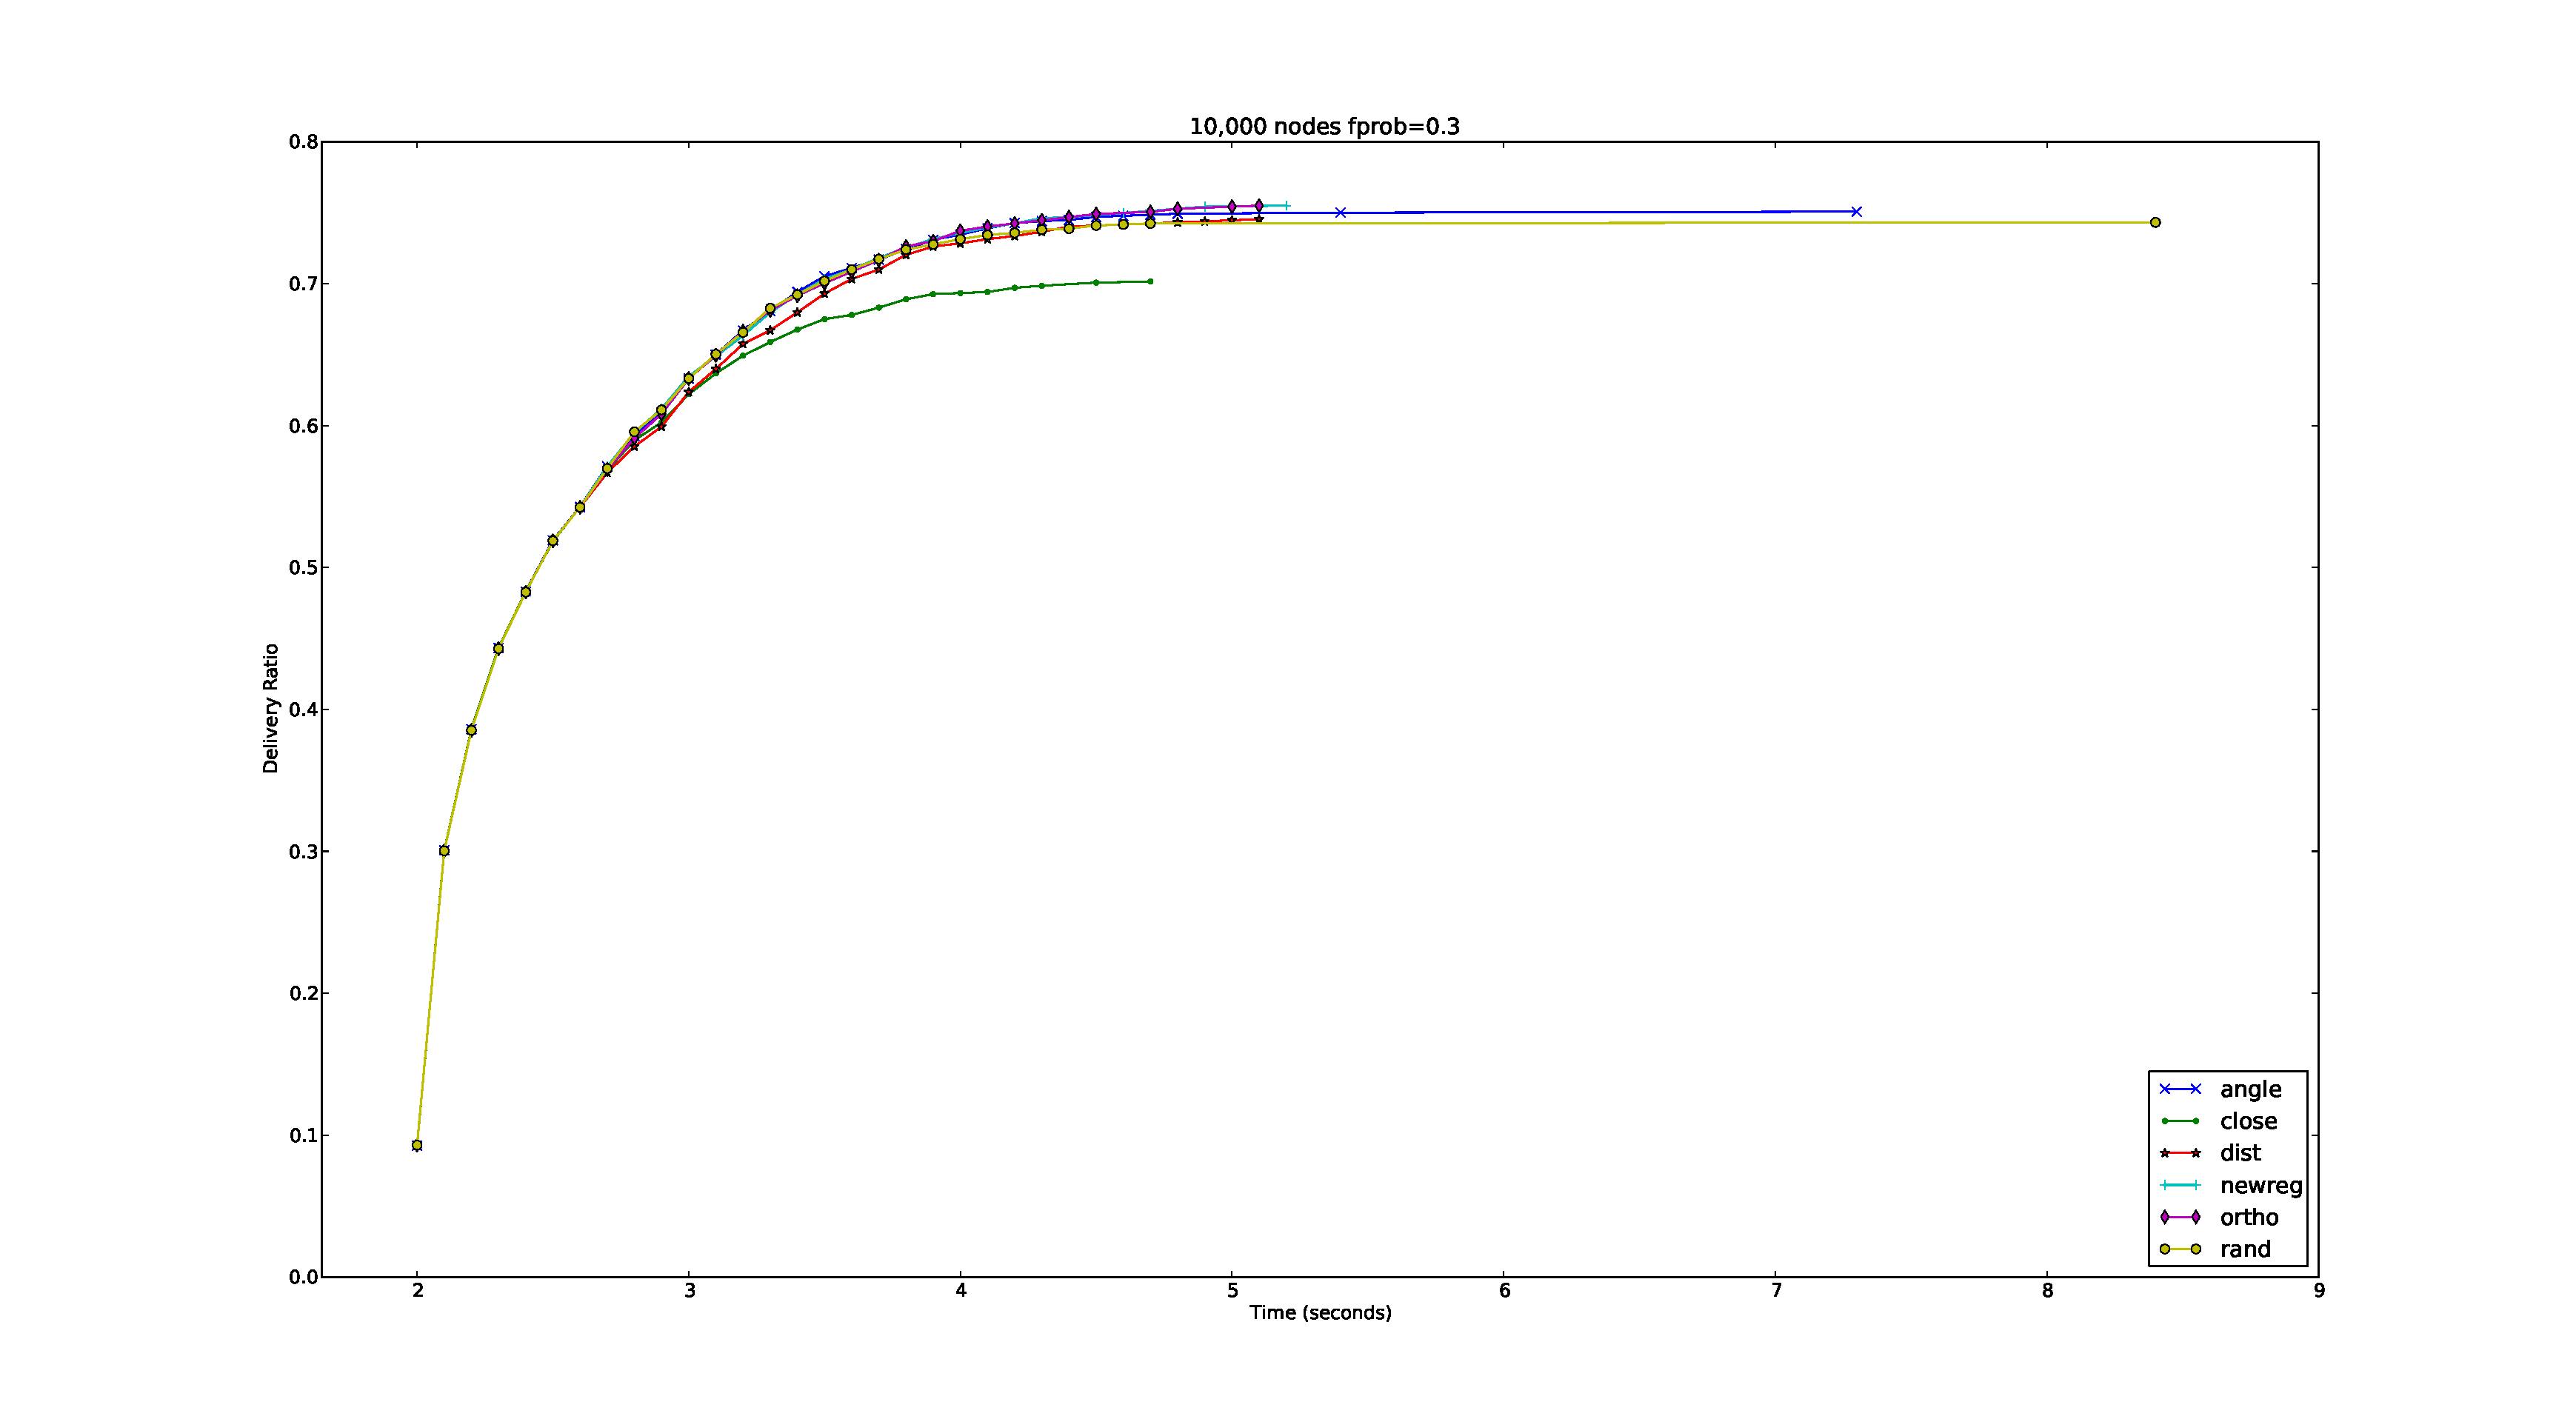
\includegraphics[width=.8\textwidth]{../../images/plots/fprob3}
\vspace{-20pt}
\caption{Delivery ratio for a failure probability of 0.3.
Note that the more restrictive heuristics stop finding alternative connections before those that pick from more diverse areas, such as Random and New Angle.
This pattern, as well as the relatively poor performance of Nearest Neighbor, grows proportionally to the failure probability.}
\end{figure}

\end{document}